\section{Results}



\subsection{Experiments}

Here we discuss comparisons we made between different models.

\subsubsection{Network depth and width} \label{sssec:exp_encoder}

By training on the simpler four-digit MNIST dataset without noise, 
%we made several observations.
% We experimented on various configurations of encoder and decoder depth and width.
we found that increasing the width of the decoder's hidden layer from 512 to 1024 had a very small impact on the training time while increasing accuracy. Decreasing the number of layers in the encoder from 7 to 5 decreased the accuracy somewhat but increased training time considerably. Halving the encoder width halved the training time but also decreased accuracy. Adding a pooling layer at the end of the encoder resulted in a higher accuracy after the first epoch and reduced training time.


\begin{figure}
    \centering
    \begin{subfigure}[c]{1.0\textwidth}
        \centering    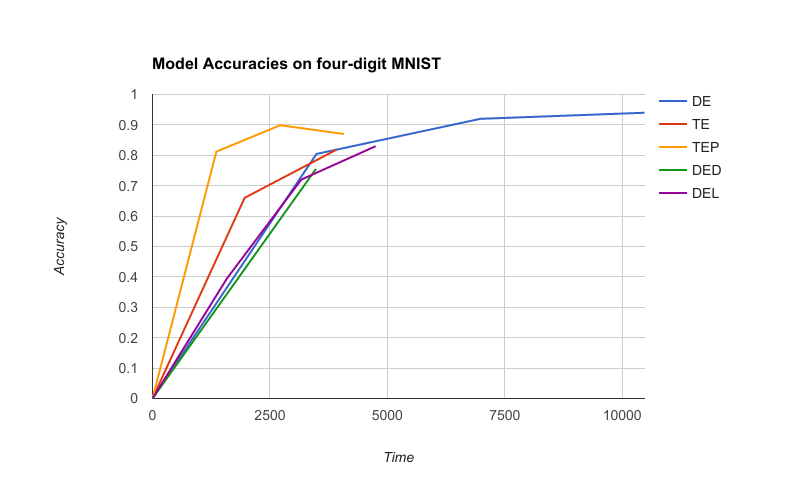
\includegraphics[scale=0.5]{resources/mnist_4_graph.png}
        \caption{Four-digit MNIST without noise.}
        \label{fig:mnist_early_models}
    \end{subfigure}
    \begin{subfigure}[c]{1.0\textwidth}
        \centering
        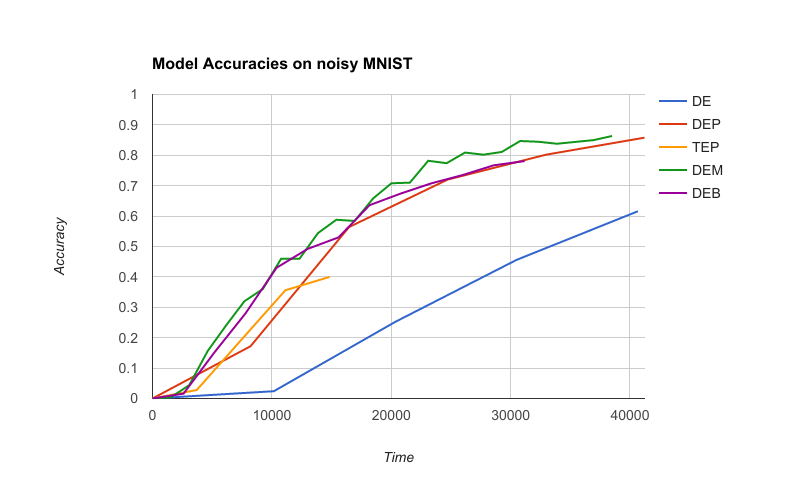
\includegraphics[scale=0.5]{resources/model_experiments.png}
        \caption{Noisy MNIST.}
        \label{fig:mnist_models}
    \end{subfigure}
    \caption{Plot of accuracy vs training time measured in CPU seconds for several models. Each data point comes after one epoch of training.}
\end{figure}


The best variations were evaluated on the more difficult synthetic dataset with random positions and noise. Figure \ref{fig:mnist_models} contains a comparison between some variations of encoder configurations on the noisy MNIST dataset. The three best model configurations (DEM, DEP, DEB) achieved very similar results considering the test accuracy vs training time.



% By training on the simpler four-digit MNIST dataset without noise, we found several viable configurations of encoder and decoder.

% We found various viable models by working on the simpler dataset of four-digit MNIST without noise.




% \subsubsection{Encoder depth}

\subsubsection{Soft vs hard attention}

\subsubsection{Independent digits} \label{sssec:ind_digits}

\subsubsection{Multi-year vs single-year loss function}
